% Nie dawajcie [ht] tylko odwołajcie się \ref w~opisie to latex to sam ładnie ułoży

\section{Analiza działania algorytmów}
% Wykresy Damian & Maja, opis Kuba
% Nie zapomnieć o~profilerze, skriny som jusz

W ramach pomiarów wydajności przeprowadzono testy na dwóch przeglądarkach, z wykorzystaniem dwóch platform sprzętowych. Z~racji na podobieństwa niektórych wyników, nie wszystkie dane opisujące różne warianty wykonania algorytmów zostały zaprezentowane w~dalszych opisach. Zwrócono jednak uwagę na istotne różnice. W~tabeli~\ref{tab:1} przedstawiono używane konfiguracje zestawów pomiarowych, do których odnosić się będą późniejszy opisy. Rozmiarem problemu jest długość przeszukiwanego tekstu. Długość wzorca jest zawsze równa 7, czyli w~zaokrągleniu tyle, ile wynosi średnia długość wyrazu w~języku polskim~\cite{Polski}. Każda seria danych wykresu średniego czasu wykonania algorytmu zawiera dodatkowo czas minimalny i maksymalny w postaci pionowych linii, a także odchylenie standardowe w postaci zacieniowanego obszaru.
\begin{table}[H]
    \centering
    \begin{tabular}{ |r l l l|  }
        \hline
        Konfiguracja & CPU                               & GPU                   & Przeglądarka    \\
        \hline
        \hline
        1.1          & Intel Core i7-4770S CPU @ 3.10GHz & Nvidia GTX 970        & Google Chrome   \\
        1.2          & Intel Core i7-4770S CPU @ 3.10GHz & Nvidia GTX 970        & Mozilla Firefox \\
        2.1          & Intel Core i5-6300U CPU @ 2.40GHz & Intel HD Graphics 520 & Google Chrome   \\
        2.2          & Intel Core i5-6300U CPU @ 2.40GHz & Intel HD Graphics 520 & Mozilla Firefox \\
        \hline
    \end{tabular}
    \caption{Konfiguracje zestawów pomiarowych}
    \label{tab:1}
\end{table}

\subsection{Wersja dla CPU -- jeden wątek}

Pierwszym przedmiotem badania jest pomiar czasu wykonania algorytmu na jednym wątku CPU. Na rysunku \ref{fig:chart_cpu_sc_mean_chrome} przedstawiono czas wykonania przy rosnącym rozmiarze problemu. Zgodnie z oczekiwaniami, przy stałym rozmiarze wzorca, złożoność algorytmu jest liniowa.
Środowisko przeglądarki internetowej, ze względu na skupienie się na obsłudze interfejsu użytkownika i asynchronicznych zadaniach, toleruje dłuższe opóźnienia. Opóźnienia te są widoczne w postaci dużego zróżnicowania czasów maksymalnych i wynikają prawdopodobnie z asynchronicznej komunikacji pomiędzy wątkami, która nie musi mieć dużego priorytetu dla przeglądarki.

% Różnice pomiędzy przeglądarkami, napomknąć o~wielu testach

\begin{figure}
    \centering
    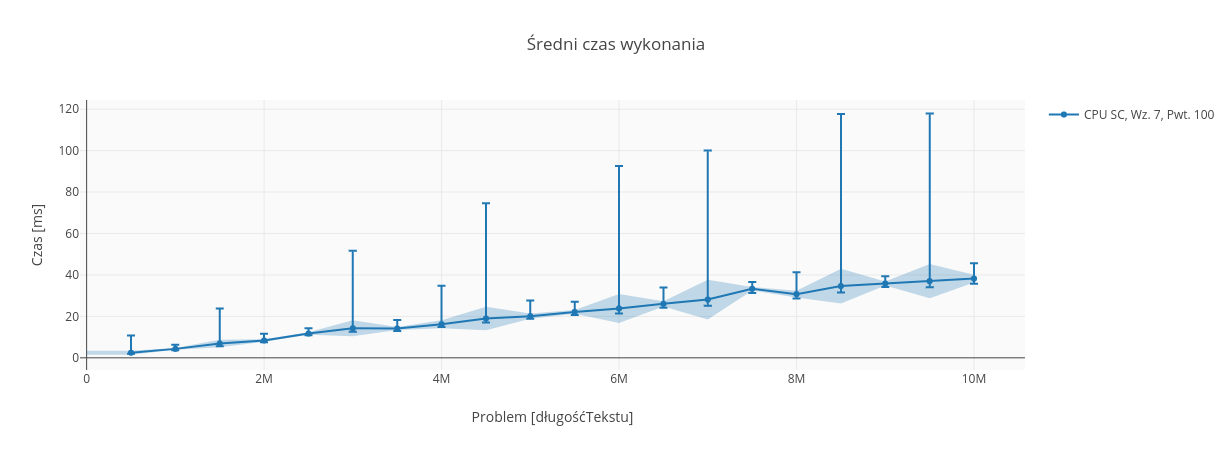
\includegraphics[keepaspectratio, width=1.0\linewidth, trim=1.1cm 0.9cm 0.5cm 3.5cm, clip]{benchmarks/nvidia970_chrome/cpu_sc_mean.png}
    \caption{Czas wykonania algorytmu CPU, jeden wątek, zestaw 1.1}
    \label{fig:chart_cpu_sc_mean_chrome}
\end{figure}


\begin{figure}
    \centering
    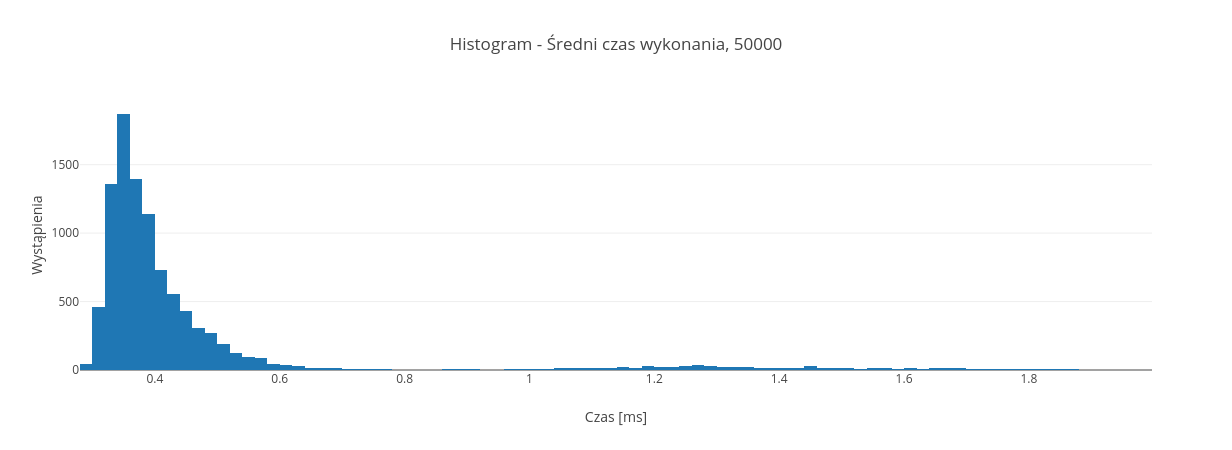
\includegraphics[keepaspectratio, width=1.0\linewidth, trim=1.1cm 0.9cm 0.5cm 3.5cm, clip]{benchmarks/nvidia970_chrome/his.png}
    \caption{Histogram czasu wykonania algorytmu CPU, problem 50.000/7, 10.000 powtórzeń, jeden wątek, zestaw 1.1}
    \label{fig:chart_cpu_sc_his_chrome}
\end{figure}

Zróżnicowanie czasu wykonania zobaczyć można dobrze na histogramie na rysunkach~\ref{fig:chart_cpu_sc_his_chrome} i~\ref{fig:chart_cpu_sc_his_firefox}. Analizując wykres dla zestawu 1.1 (Google Chrome) widać, że czas w~zdecydowanej większości oscyluje w~okolicach $0.4$~ms, ale część wyników pojawia się również w~zakresie $1.2-1.4$~ms. Przeglądarka Mozilla Firefox (rysunek~\ref{fig:chart_cpu_sc_mean_firefox} i~\ref{fig:chart_cpu_sc_his_firefox}) okazała się być mniej wydajna. Dla małych czasów wykonania istotny może być fakt, że ze względów bezpieczeństwa Mozilla Firefox ma ograniczoną precyzję pomiaru czasu z~użyciem interfejsu \texttt{Performance}.


\begin{figure}
    \centering
    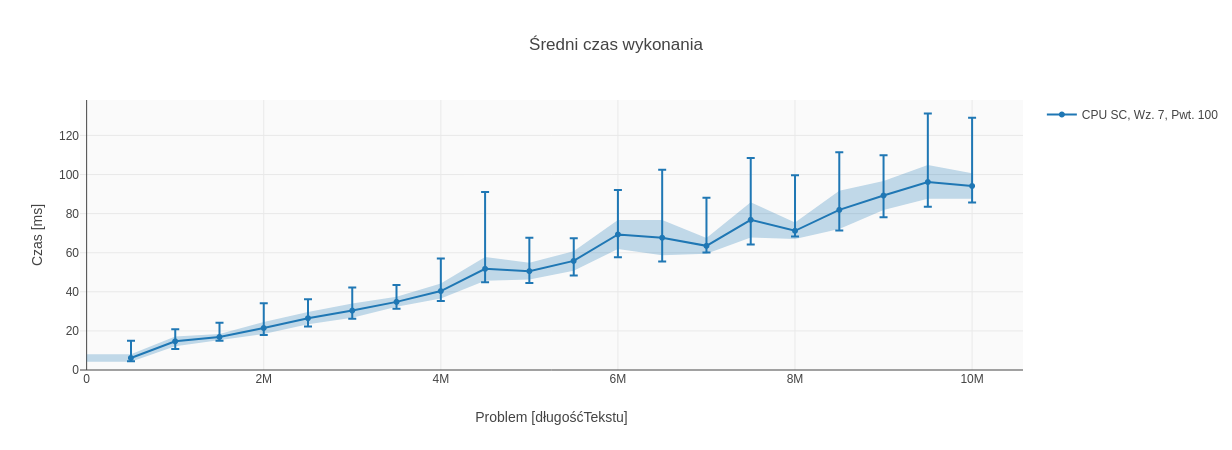
\includegraphics[keepaspectratio, width=1.0\linewidth, trim=1.1cm 0.9cm 0.5cm 3.5cm, clip]{benchmarks/nvidia970_firefox/cpu_sc_mean.png}
    \caption{Czas wykonania algorytmu CPU, jeden wątek, zestaw 1.2}
    \label{fig:chart_cpu_sc_mean_firefox}
\end{figure}

\begin{figure}
    \centering
    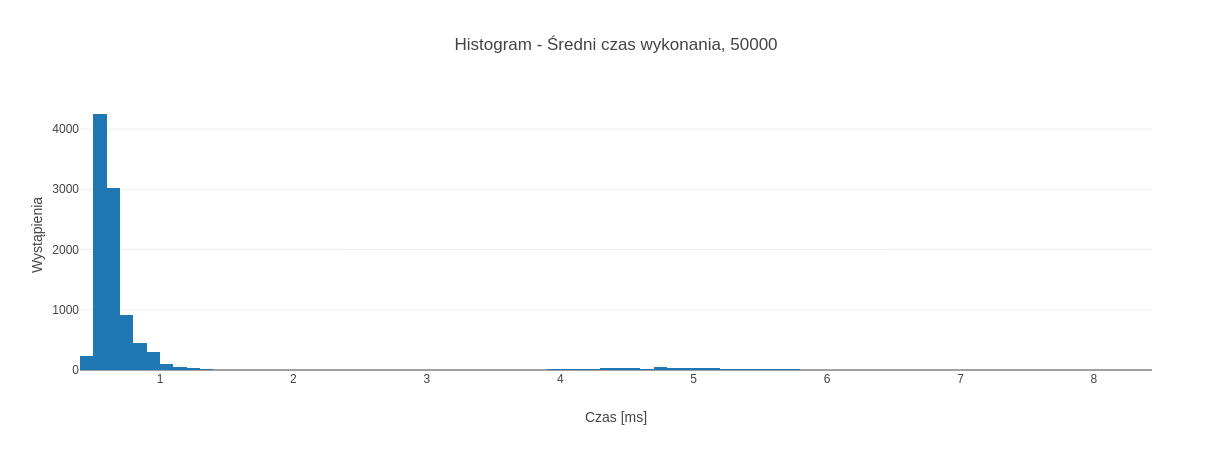
\includegraphics[keepaspectratio, width=1.0\linewidth, trim=1.1cm 0.9cm 0.5cm 3.5cm, clip]{benchmarks/nvidia970_firefox/his.png}
    \caption{Histogram czasu wykonania algorytmu CPU, problem 50.000/7, 10.000 powtórzeń, jeden wątek, zestaw 1.2}
    \label{fig:chart_cpu_sc_his_firefox}
\end{figure}

\subsection{Wersja dla CPU -- wiele wątków}
% - porównać diagramy Mai i~Damiana (2(4)Core vs 4(8)Core)

Kolejno zbadano pomiar czasu wykonania przy podziale podzadań wyszukiwania na wiele wątków. Na rysunkach~\ref{fig:chart_cpu_mc_mean_chrome_damian} i~\ref{fig:chart_cpu_mc_mean_chrome_maja} przedstawiono wyniki pomiaru czasu wykonania dla różnej liczby wątków. Zestaw 1.1 posiada czterordzeniowy CPU i na wykresie widoczne jest, że czas wykonania maleje względem wykonania jednowątkowego dla dwóch i czterech wątków. Dalsze zwiększanie liczby wątków nie przynosi przyspieszenia.
Zestaw 2.1 posiada dwurdzeniowy CPU i w tym przypadku zysk w postaci czasu wykonania widać tylko dla dwóch wątków.


\begin{figure}
    \centering
    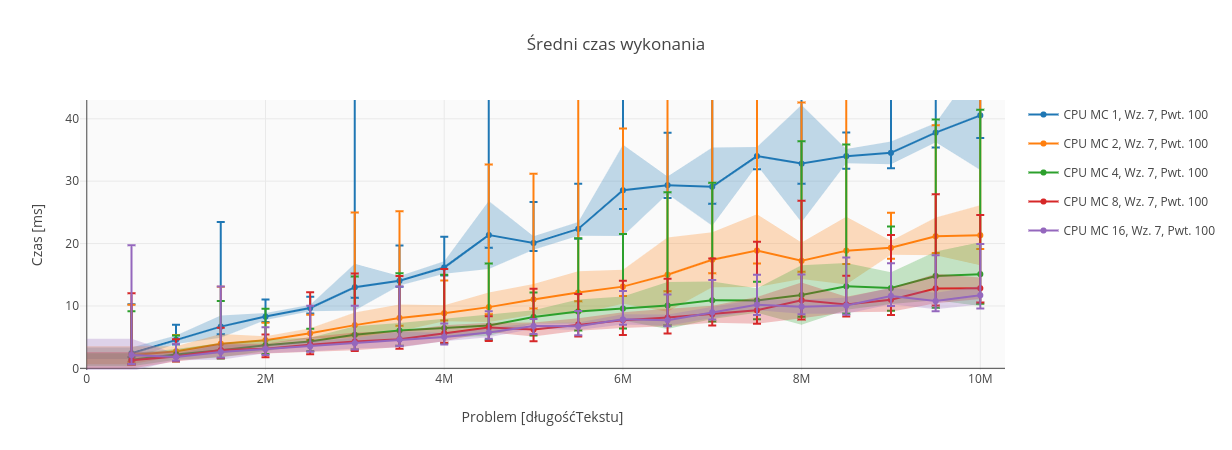
\includegraphics[keepaspectratio, width=1.0\linewidth, trim=1.1cm 0.9cm 0.5cm 3.5cm, clip]{benchmarks/nvidia970_chrome/cpu_mc_mean_zoom.png}
    \caption{Czas wykonania algorytmu CPU Multi Core, zestaw 1.1}
    \label{fig:chart_cpu_mc_mean_chrome_damian}
\end{figure}

\begin{figure}
    \centering
    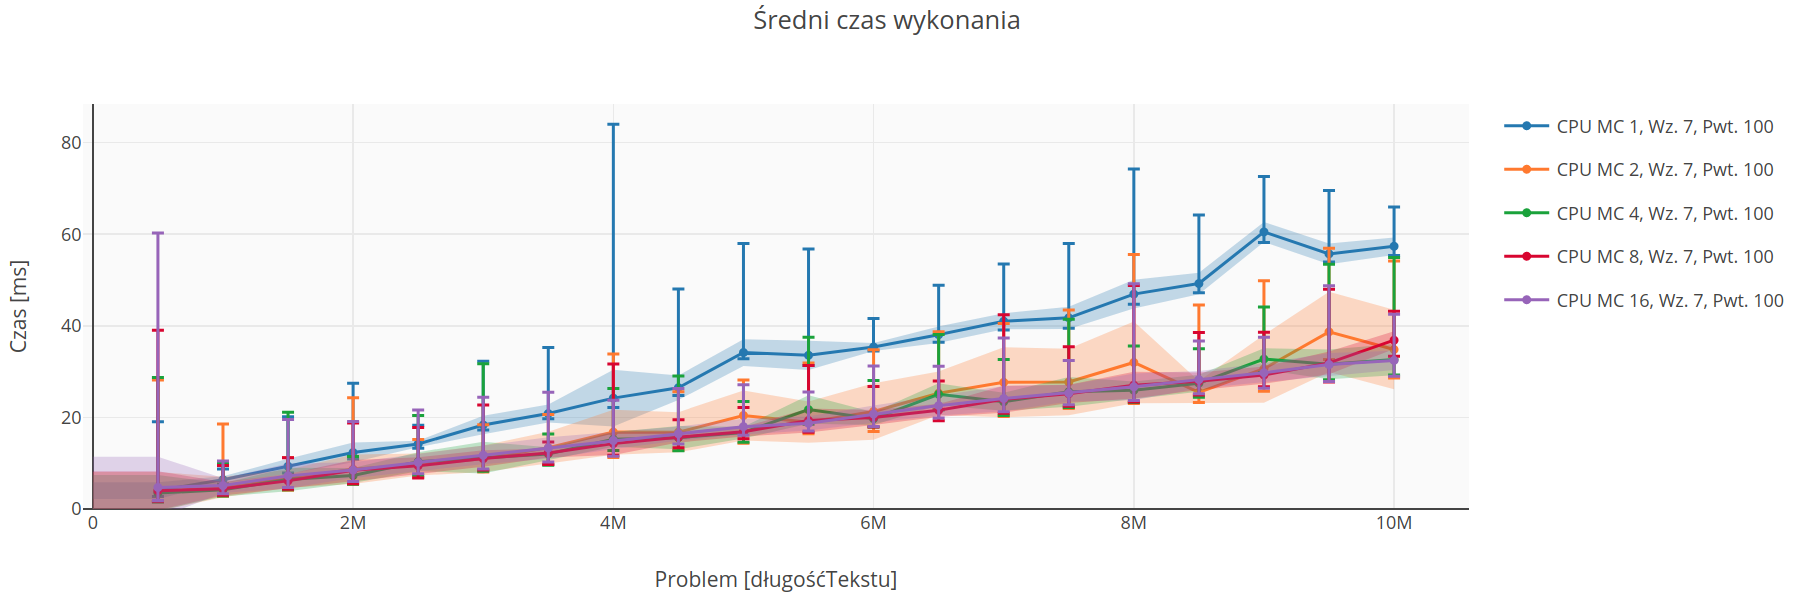
\includegraphics[keepaspectratio, width=1.0\linewidth, trim=0 0 0 2.7cm, clip]{benchmarks/intel_hd520_chrome/cpu_mc_mean.png}
    \caption{Czas wykonania algorytmu CPU Multi Core, zestaw 2.1}
    \label{fig:chart_cpu_mc_mean_chrome_maja}
\end{figure}

Na rysunku~\ref{fig:profiler_cpu} zamieszczono wycinek graficznej reprezentacji analizy profilera przeglądarki Google Chrome wykonania algorytmu na dwóch wątkach. Można zauważyć, że pierwsze wykonanie jest z reguły wolniejsze od pozostałych.

\begin{figure}
    \centering
    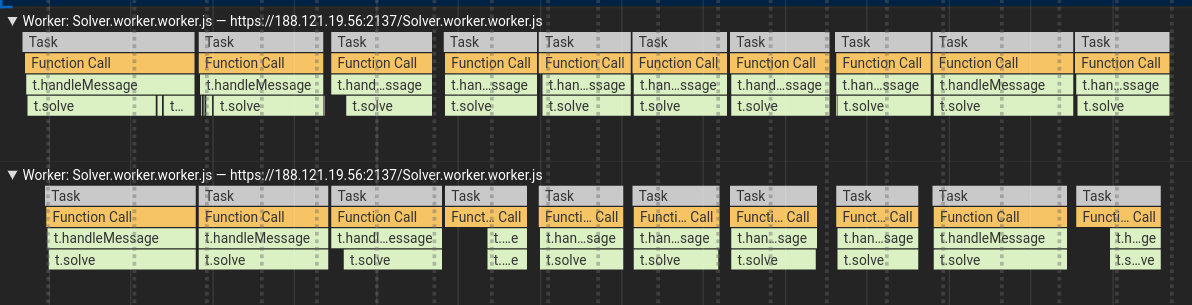
\includegraphics[keepaspectratio, width=1.0\linewidth]{benchmarks/nvidia970_chrome/cpu_2_profiler.png}
    \caption{Analiza wykonania algorytmu CPU, zestaw 1.1}
    \label{fig:profiler_cpu}
\end{figure}


\subsection{Wersja dla GPU}
% - dlaczego wyszło jak wyszło
% - rozmiar problemu rośnie razem z~wynikiem
% - tutaj dać te wzorki w~porównaniu do macierzy i~porównać do macierzy

% - dużo zajmuje pobranie wyniku
% - dużo zajmuje interpretacja wyniku (filter)


Celem w zadaniu akceleracji dla wyszukiwania wzorca (o stałej długości) w tekście, w przypadku algorytmu naiwnego jest osiągnięcie złożoności poniżej $\mathcal{O}(n)$; docelowo $\mathcal{O}(1)$ dla przypadków nie wykraczających poza możliwości karty graficznej. Niestety, jak widać na rysunkach \ref{fig:chart_gpu_mean_chrome_damian} oraz \ref{fig:chart_gpu_mean_chrome_maja} algorytm uruchomiony na GPU charakteryzuje się liniową zależnością czasu wykonania od rozmiaru problemu bez względu na konfigurację sprzętową. Tak, jak w przypadku CPU zauważalna jest niestabilność środowiska przeglądarki, co wpływa na duży rozrzut uzyskanych pomiarów czasu wykonania, jednak w przypadku GPU rozrzut tej jest zauważalnie mniejszy. Może to wynikać z faktu, iż przeglądarka nie przydziela zadań GPU tak niedeterministycznie, jak w przypadku CPU.

Ciekawy okazuje się rozkład całkowitego czasu wykonania algorytm na jego części składowe, który można zaobserwować na rysunku \ref{fig:profiler_gpu} przedstawiającym dane narzędzia profilującego wbudowanego w przeglądarkę. Jak się okazuje, kluczowy jest udział podzadań w całkowitym czasie wyszukiwania. Całkowity czas zadania z pominięciem stałych jest oznaczony na rysunku \ref{fig:profiler_gpu} jako \textit{t.solve}. Kluczowe składowe to: 
\begin{enumerate}
    \item wykonanie obliczeń na GPU - element \textit{run},
    \item odczytanie bufora GPU - element \textit{readPixels},
    \item konwersja wyjścia GPU do formatu gęstego (lista indeksów tekstu pasującego do wzorca) - czas pomiędzy zakończeniami \textit{readPixels} i \textit{t.solve}.
\end{enumerate}
Po zbadaniu danych narzędzia profilującego dla algorytmu wyszukiwania na GPU okazuje się, że elementy te mają udział w ogólnym czasie wykonania \textit{t.solve}:
\begin{itemize}
    \item dla właściwych obliczeń - 5\%,
    \item dla odczytania bufora GPU - 20\%,
    \item dla operacji przetworzenia danych wyjściowych z GPU - 75\%.
\end{itemize}
Dzieje się tak, gdyż obliczenia dla jednego wątku GPU nie są wymagające pod względem czasu. Uwidaczniają się tutaj problemy akceleracji obliczeń: gdy czas kopiowania danych jest znacznie większy od czasu wykonywanych obliczeń, trudno jest osiągnąć przyspieszenie. Dla konkretnego przypadku tego algorytmu w połączeniu z freamworkiem GPU.js, od którego zależy wymaganie czasowe funkcji \textit{readPixels()} okazuje się, iż uzyskanie akceleracji jest dodatkowo utrudnione, gdyż wyniki poszczególnych wątków są czytane sekwencyjnie. Implementacja algorytmu na GPU przydziela każdemu wątkowi GPU indeks w potencjalnie dużym tekście, co sprawia, że wyników do sekwencyjnego odczytania jest dużo -- uwidacznia się to w stosunku czasów wykonania 4:1 pomiędzy operacją odczytania wyników GPU, a właściwymi obliczeniami.

Nietrudno też zauważyć znaczną dominację czasową przetworzenia danych wynikowych z GPU przez CPU. Format wyjścia GPU jest z góry narzucony, dlatego aby uzyskać akcelerację należy zastanowić się nad koniecznością wykonywania konwersji. Jeżeli nie wymagają tego zależności zewnętrzne, konwersje wyjścia GPU powinny zostać wyeliminowane -- w przeprowadzonych badaniach konwersja taka zajęła trzykrotnie więcej czasu niż samo przetwarzanie na GPU.

\begin{figure}
    \centering
    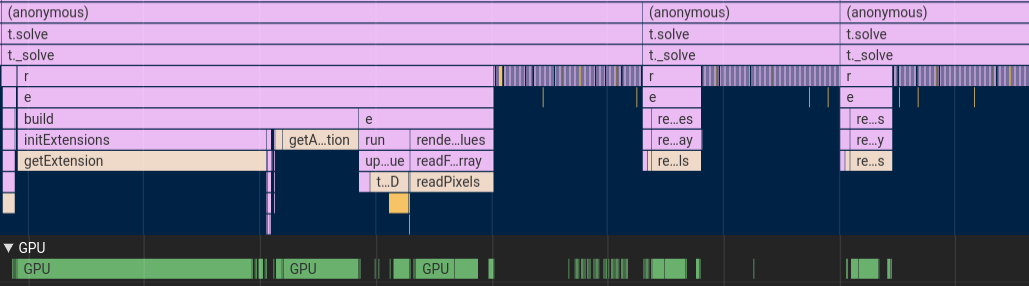
\includegraphics[keepaspectratio, width=1.0\linewidth]{benchmarks/nvidia970_chrome/gpu_profiler.png}
    \caption{Analiza wykonania algorytmu GPU, zestaw 1.1}
    \label{fig:profiler_gpu}
\end{figure}

\begin{figure}
    \centering
    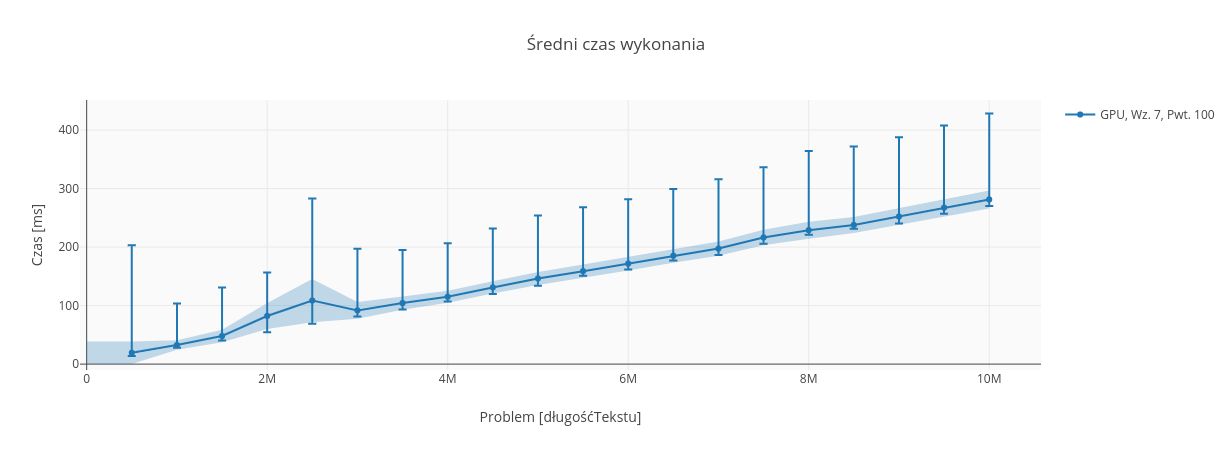
\includegraphics[keepaspectratio, width=1.0\linewidth, trim=1.1cm 0.9cm 0.5cm 3.5cm, clip]{benchmarks/nvidia970_chrome/gpu_mean.png}
    \caption{Czas wykonania algorytmu GPU, zestaw 1.1}
    \label{fig:chart_gpu_mean_chrome_damian}
\end{figure}

\begin{figure}
    \centering
    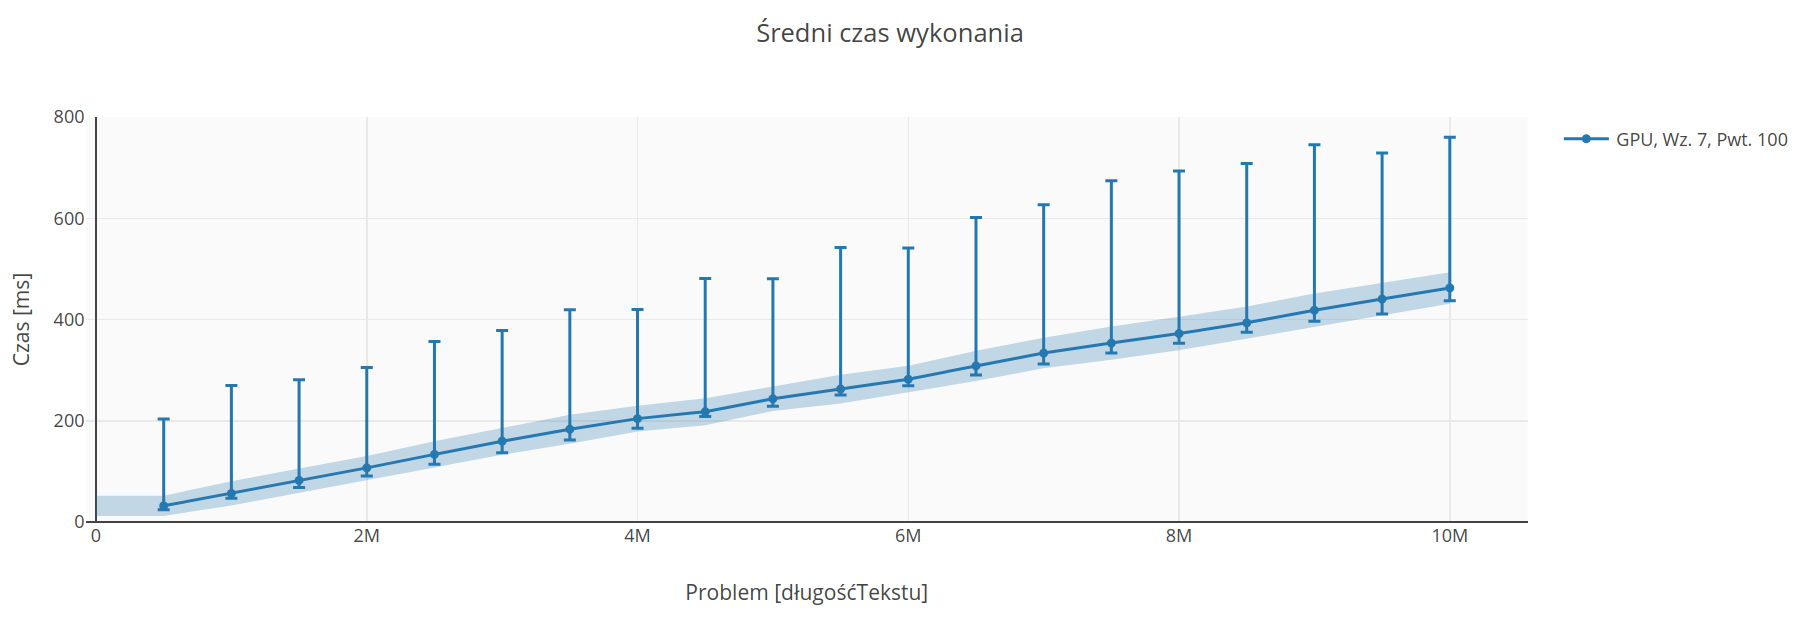
\includegraphics[keepaspectratio, width=1.0\linewidth, trim=0 0 0 2.7cm, clip]{benchmarks/intel_hd520_chrome/gpu_mean.png}
    \caption{Czas wykonania algorytmu GPU, zestaw 2.1}
    \label{fig:chart_gpu_mean_chrome_maja}
\end{figure}

\subsection{Zestawienie}
% rzeczy z~taba w~UI - Podsumowanie

Na rysunkach \ref{fig:chart_summary_chrome_damian} oraz \ref{fig:chart_summary_chrome_maja} zestawiono czasy wykonania algorytmu na CPU oraz GPU. Można zauważyć, iż konfiguracja sprzętowa nie odgrywa tutaj znaczącej roli -- z dokładnością do stałej obie wersje algorytmów mają tą samą charakterystykę czasową niezależnie od platformy sprzętowej.

W przedstawionej skali uwzględniającej średni przypadek wyszukiwania wzorca w tekście można zauważyć, iż wyniki są odwrotne do spodziewanych. Algorytm dla GPU wraz ze wzrostem długości tekstu, liniowo zwiększa czas potrzebny na obliczenie wyniku -- czas jego wykonania jest rządu 100 ms, co może być zauważalne dla użytkownika. Dla CPU sytuacja jest odwrotna; mimo, iż CPU charakteryzuje się obliczeniami sekwencyjnymi, to nawet dla naiwnego wyszukiwania wzorca w tekście można przyjąć, iż czas wykonania algorytmu jest stały w rozważanej skali. Wiadomo z rysunku \ref{fig:chart_cpu_sc_mean_chrome}, że algorytm ten ma w przybliżeniu złożoność liniową, jednak zmiana rzędu 10 ms byłaby niezauważalna dla użytkownika.

Sytuacja ta może wynikać z faktu, iż wraz ze wzrostem rozmiaru problemu (w tym przypadku długości tekstu) wymagane jest przydzielenie kolejnych wątków obliczeniowych na GPU, co zwiększa liczbę danych do późniejszego odczytania z bufora GPU i przekonwertowania do ustalonego formatu. Operacje transferu danych są na GPU kosztowne. W przypadku CPU problem ten nie występuje i pomimo swojej sekwencyjnej natury problem wyszukiwania naiwnego jest przez CPU rozwiązywany znacznie efektywniej.

\begin{figure}
    \centering
    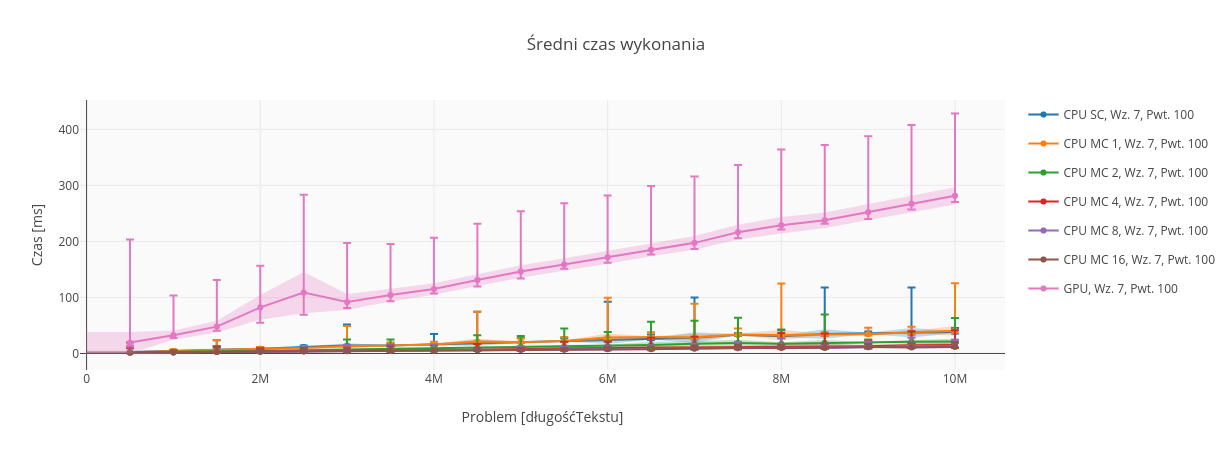
\includegraphics[keepaspectratio, width=1.0\linewidth, trim=1.1cm 0.9cm 0.5cm 3.5cm, clip]{benchmarks/nvidia970_chrome/summary_mean.png}
    \caption{Podsumowanie czasów wykonania algorytmu, zestaw 1.1}
    \label{fig:chart_summary_chrome_damian}
\end{figure}

\begin{figure}
    \centering
    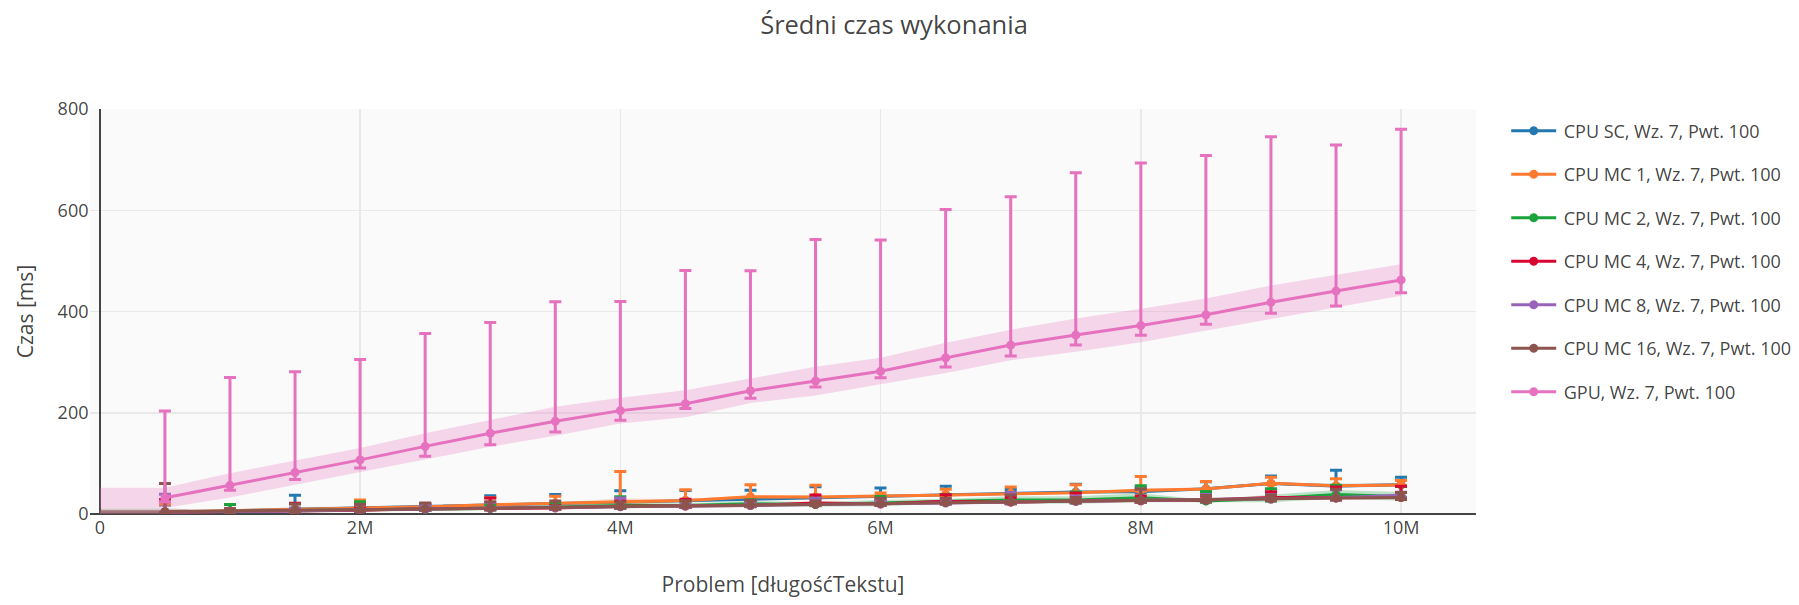
\includegraphics[keepaspectratio, width=1.0\linewidth, trim= 0 0 0 2.7cm, clip]{benchmarks/intel_hd520_chrome/summary_mean.png}
    \caption{Podsumowanie czasów wykonania algorytmu, zestaw 2.1}
    \label{fig:chart_summary_chrome_maja}
\end{figure}